\section{Architecture}
\label{qoala:sec:architecture}

Based on these design considerations, we propose Qoala (see \cref{qoala:fig:runtime_overview}), an execution environment for programmable nodes in a quantum internet. 
Provided minimal hardware assumptions are met (\cref{qoala:sec:minimal_hardware_assumptions}), 
each node implements its own Qoala execution environment, supporting a specific \textit{program structure} (\cref{qoala:sec:program_structure})
and implementing a specific \textit{runtime environment} (\cref{qoala:sec:runtime_environment}) that is able to \textit{schedule tasks} (\cref{qoala:sec:tasks,qoala:sec:program_instantiation,qoala:sec:scheduling}).
Details in \cref{qoala:sec:app:program_structure,qoala:sec:app:runtime_environment,qoala:sec:app:scheduling_execution}.

\subsection{Minimal hardware assumptions}
\label{qoala:sec:minimal_hardware_assumptions}

Qoala is based on only a few core assumptions on the processing node (consideration EC3, \cref{qoala:fig:minimal_hardware_assumptions}):

\textit{CPS-QPS distinction}. We assume the node distinguishes between a \textit{classical processing system (CPS)} managing classical computing resources (e.g. CPU, classical memory and networking), and a \textit{quantum processing system (QPS)}, responsible for executing quantum operations (gates, measurements, entanglement generation) on quantum hardware including a quantum memory as in \cref{chp:netqasm,chp:qnodeos}.
We hence use a similar distinction as with the CNPU and QNPU from \cref{chp:netqasm,chp:qnodeos} but with a slightly different terminology and division of abstractions:
the CPS is on the same level as the CNPU from \cref{chp:netqasm,chp:qnodeos}, but the QPS is either just the QNPU level or the combined `QNPU + QDevice' level.
Unlike in the implementation of QNodeOS, we assume a shared classical memory is accessible to both the CPS and QPS, enabling communication between the two processing systems, addressing the interactive property of quantum internet programs.
The CPS can act as a fully-fledged classical computer, and performs application-level classical communication with other nodes as well as with a network controller who sets a network schedule.
The QPS can execute routines consisting of low-level quantum gates, basic classical control logic (branching), and entanglement generation.
This opens the door for the QPS to be based on essentially any quantum hardware platform where a specialized microcontroller is used to control the quantum hardware, and a separate microprocessor implements the CPS, where a shared memory could be realized next to the two processors on-chip.
The scheduler controls both CPS and QPS execution, and may physically be realized on either one.

\textit{Time granularity}. Both CPS and QPS are assumed to have knowledge of time, albeit operating with different timing precision ($ms$ precision for CPS mirroring node-to-node communication latencies vs. $\mu s$ and $ns$ precision needed for synchronized entanglement generation~\cite{pompili2022experimental, dahlberg2019link}.)

 \textit{Network stack}. A quantum network stack including a network layer~\cite{dahlberg2019link} is implemented on the node with which Qoala can interface. This stack can receive and fulfill requests for remote entanglement generation.
\begin{figure}
    \centering
    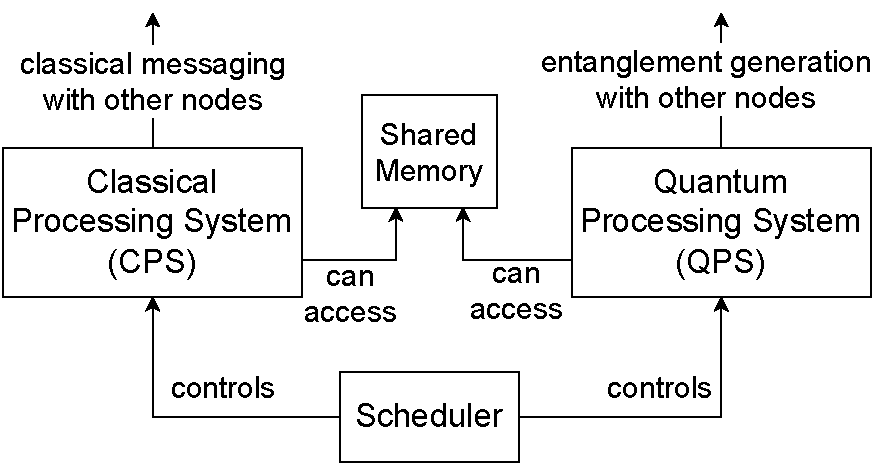
\includegraphics[width=0.7\textwidth]{figures/qoala/minimal-hardware.pdf}
    \caption{Minimal hardware assumptions for a single node.
    A Classical Processing System (CPS) can execute classical code and can communicate classical messages with other nodes in the network.
    A Quantum Processing System (QPS) can execute quantum code and can realize entanglement (quantum connections) with other nodes in the network.
    The CPS and QPS are controlled by a scheduler, and have access to shared memory.
    In the QNodeOS architecture~\cite{qnodeos_nature}, the CPS is realized as the CNPU, and the QPS as the combined QNPU-QDevice system.
    For Qoala, we only focus on the classical-quantum distinction, and not the internal implementation (such as a QNPU-QDevice separation), hence the different terminology.
    }
    \label{qoala:fig:minimal_hardware_assumptions}
\end{figure}



\subsection{Program structure}
\label{qoala:sec:program_structure}
Qoala defines a hybrid format for programs, mapping naturally to their hybrid nature (consideration FC1 in \cref{qoala:sec:design_considerations}).
A Qoala program is a combination of quantum and classical instructions, 
organized into three main sections: \textit{host code} (containing classical instructions), \textit{local routines} (containing local quantum instructions), 
and \textit{request routines} (for remote entanglement generation).
This hybrid format allows a compiler to optimize the whole program, including critical code paths with dependencies between classical and quantum segments.
Local routines and request routines can be triggered from within host code as function calls, addressing the interactivity between them (consideration FC2).

A Qoala program is an \textit{executable} and output of a compiler.
The format is separate from any high-level language in which a programmer might write code; hence Qoala in theory allows for compatibility with any such language (consideration EC1).
Entry and exit points of a program are in host code.
\cref{qoala:fig:example_program} shows an example program in text format.
We contrast Qoala's program format with that of NetQASM (see~\cite{dahlberg2022netqasm} and \cref{chp:netqasm,chp:qnodeos}), in which there was no way to compile across classical and quantum code segments.
A Qoala program has \textit{program arguments} that are filled in during program instantiation (\cref{qoala:sec:program_instantiation}).


\begin{figure}
    \centering
    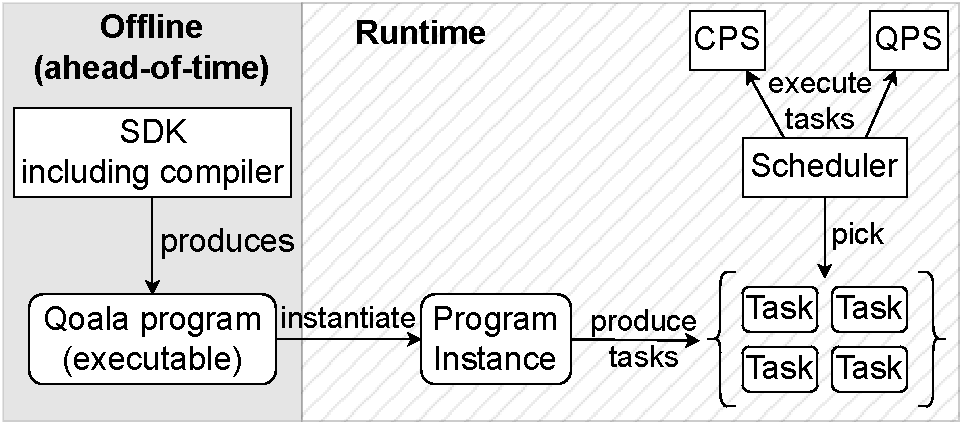
\includegraphics[width=0.7\textwidth]{figures/qoala/runtime_overview.pdf}
    \caption{High-level overview Qoala: An SDK allows program code in a high-level language (e.g. Python).
    A compiler translates this code into a Qoala program (specific compiler not in scope of this work).
    To run, a program is instantiated with concrete values for program arguments.
    Tasks are created for the program instance, which are scheduled and executed by the scheduler.
    Multiple program instances may exist at the same time (both multiple instances of the same or different programs).
    All tasks from all instances are added to a single task graph (\cref{qoala:sec:tasks}) used by the scheduler.
    }
    \label{qoala:fig:runtime_overview}
\end{figure}




\textit{Host code}.
Host code, executed on the CPS, encompasses local computation, control-flow, inter-node messaging, and can initiate local and request routines.
For example, in a program that is part of a QKD application, classical post-processing (including sending bases, local error correction, and privacy amplification \cite{vidick2023introduction}) would be represented in host code.
Host code is structured as a sequence of \textit{blocks}, each holding a list of instructions.
Blocks dictate control-flow by ending with a (conditional) jump instruction (default: next block in the sequence).
This block division not only facilitates task creation and scheduling (see \cref{qoala:sec:tasks}) but also streamlines compiler integration (which may use blocks in its intermediate representation).
Blocks can contain metadata about their expected \textit{duration}, (relative) deadlines, and they may be inside \textit{critical sections}, encompassing a sequence of blocks with a maximally allowed execution duration. This metadata is propagated to corresponding tasks and used by the scheduler in order to mitigate quantum decoherence due to limit qubit lifetime (consideration TC1).
Asynchronous execution is possible by `submitting' multiple routines for execution, and waiting for all of them to finish. At runtime, the scheduler can decide in which order to execute the routines.


\textit{Local routine}.
A local routine (LR) represents a series of quantum operations (like gates and measurement), to be executed by the QPS locally (no interaction with external nodes or controllers).
An LR may also contain limited classical computation and control-flow code allowing for fast feedback, which can increase quantum performance (\cref{qoala:sec:background_context}) due to less decoherence.
An updated version of NetQASM (see~\cite{dahlberg2022netqasm} and \cref{chp:netqasm}) is used to represent the instructions, which allows both hardware-specific and hardware-agnostic instructions.
Therefore, the program format is compatible with different quantum hardware.
In contrast to \cite{dahlberg2022netqasm}, Qoala's version of NetQASM does not have instructions for entanglement generation (cleanly separating local and networked quantum operations)
nor `wait' instructions. This allows routines to be treated as atomic non-preemptable blocks.
%, which makes scheduling easier).

\textit{Request routine}. A request routine (RR) consists of a request for entanglement generation with another node, and represent requests to the node's quantum network stack.
It can have local routines as callbacks, allowing quick local (quantum) processing of entangled qubits on the QPS without returning to the CPS, decreasing waiting time and decoherence.


\subsection{Runtime environment}
\label{qoala:sec:runtime_environment}
The Qoala runtime environment provides various resources that programs can leverage during execution.

\textit{Exposed Hardware Interface (EHI)}.
The Exposed Hardware Interface provides information about the hardware and software capabilities and restrictions of the node and the network,
like available quantum memory and expected latencies.
Each node provides their own EHI which is used in capability negotiation (see below), and allows a choice of executable code optimized by a compiler for those capabilities ahead of time. 

\textit{Shared memory}.
To address the classical-quantum interactivity in programs, the CPS and QPS share data with each other via \textit{shared classical memory}.
Write conflicts are avoided by explicit read/write rules for shared memory regions (\cref{qoala:sec:app:shared_memory}).
Our conceptual model of a shared memory leaves open different implementation choices, including a physical shared memory or a message-passing protocol.
Calls in host code to local or request routines use the shared memory to communicate routine arguments and results.

\textit{Quantum memory}.
Quantum memory is organized into a \textit{virtual quantum memory space (VQMS)} for each program instance (see \cref{qoala:sec:program_instantiation} for instantiation), represented as Unit Modules (specifying the qubit topology~\cite{dahlberg2022netqasm}).
Qoala maps each VQMS to the physical qubits available in the QPS.
VQMS information like qubit connectivity and noise characteristics is provided by the EHI, which a compiler can use to optimize a program.
The VQMS enables multitasking since programs have their own runtime context, while a scheduler (\cref{qoala:sec:scheduling}) sees the whole physical memory space and can schedule programs accordingly.

\textit{Remote interaction}. For interaction with programs on remote nodes,
the runtime provides \textit{classical sockets} and \textit{EPR sockets} based on~\cite{dahlberg2022netqasm}. Host code uses classical sockets for sending and receiving messages; EPR sockets are indicated in request routines (see e.g. \cref{qoala:fig:example_program}).

\begin{figure}
    \centering
    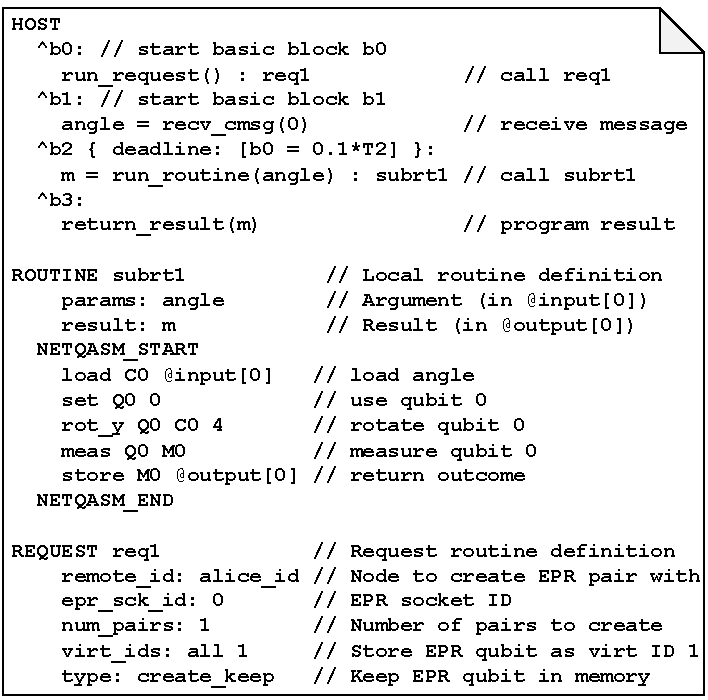
\includegraphics[width=0.6\textwidth]{figures/qoala/example_program.pdf}
    \caption{
        Example Qoala program containing a host section with 4 blocks, a local routine (\texttt{subrt1}),
        and a request routine (\texttt{req1}). Block \texttt{b2} has a relative deadline to \texttt{b0} of $0.1$ times qubit noise parameter $T_2$.
    }
    \label{qoala:fig:example_program}
\end{figure}

\begin{figure*}
    \newcommand{\figheight}{6.5cm}
    \centering
    \subfloat[\centering \label{qoala:fig:task_types}]{{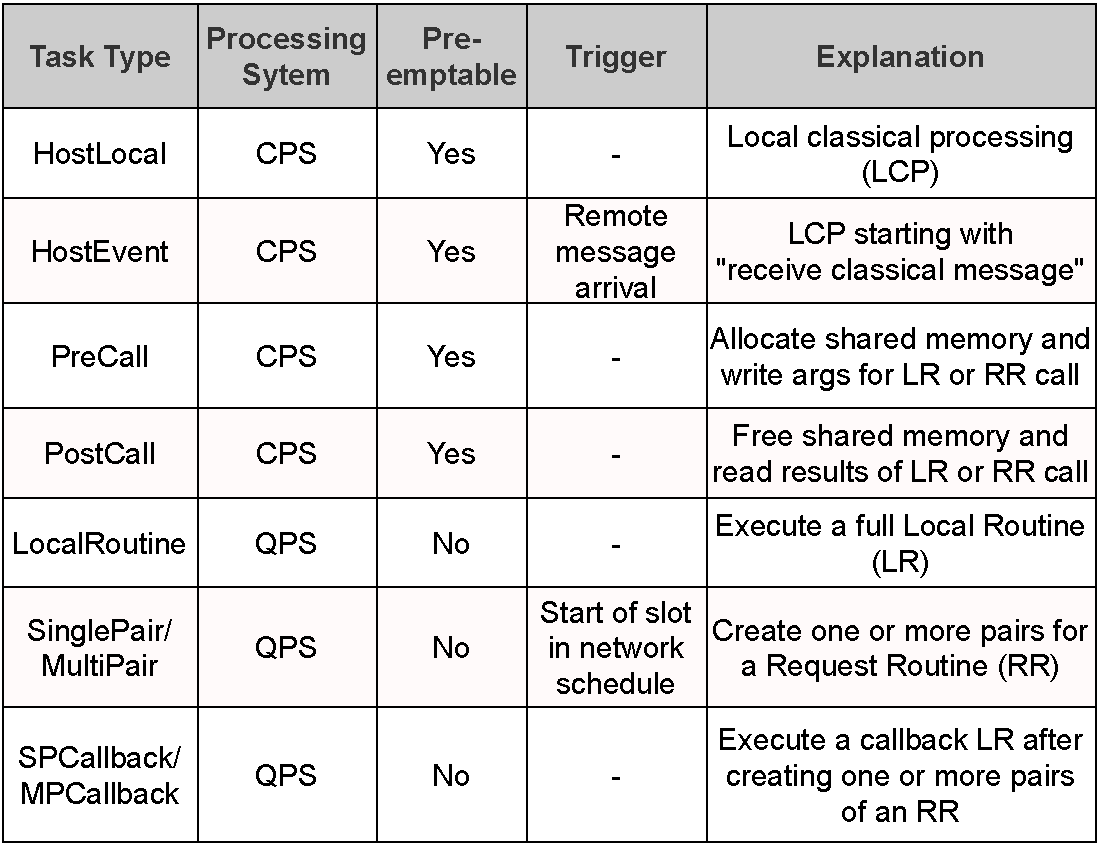
\includegraphics[height=\figheight, keepaspectratio]{figures/qoala/task-types-table.pdf}}}%
    \hfill
    \subfloat[\centering \label{qoala:fig:task_creation_cutout}]{{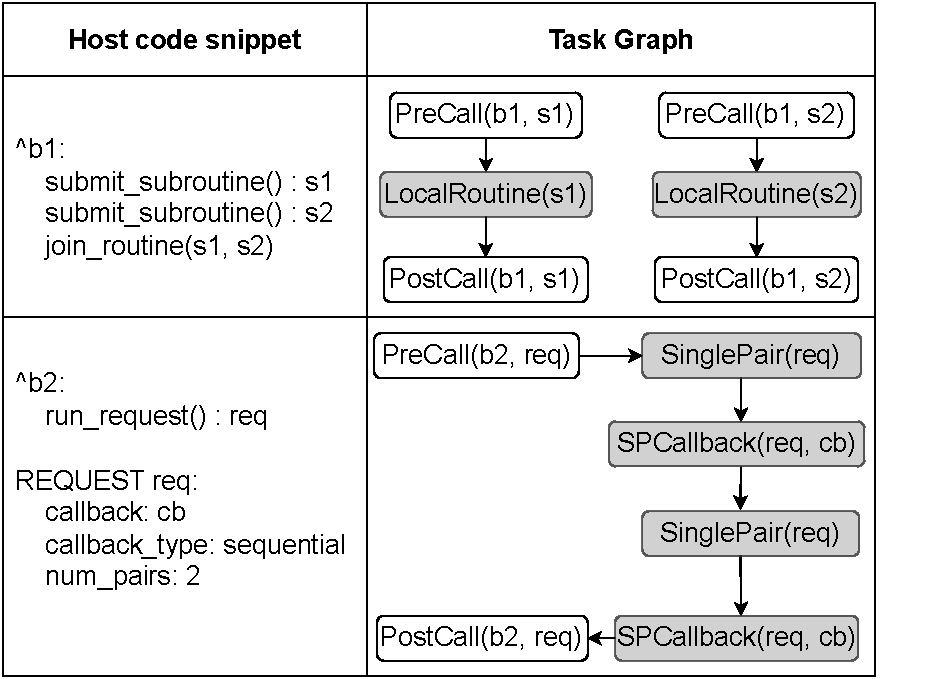
\includegraphics[height=\figheight, keepaspectratio]{figures/qoala/task_creation_cutout.pdf}}}%
    \caption{
        (a) Overview of task types.
        (b) Examples of host code and corresponding task graphs.
        Shaded tasks are executed by the QPS, the others by CPS.
        Top: asynchronous submission of local routines \texttt{s1} and \texttt{s2}.
        The graph consists of two separate chains of tasks and the scheduler can choose in which order to execute these chains (possibly interleaved).
        Bottom: a request routine uses the callback entry to immediately add tasks for executing local routine \texttt{cb} after each entangled pair generation.
    }%
    \label{qoala:fig:tasks}
\end{figure*}

\subsection{Tasks}
\label{qoala:sec:tasks}
We introduce \textit{tasks} to enable multitasking (consideration FC3).
Each task represents a code segment of a running program with a context of runtime variables.
Tasks have different types (\cref{qoala:fig:tasks}) based on the code they represent.
By splitting a program into distinct executable tasks, 
we can utilize the parallel execution on the CPS and QPS (by assigning tasks to the corresponding system),
and we can interleave execution of multiple programs by filling waiting times of one program by execution of tasks of another.
Code segments indicated to run asynchronously (\cref{qoala:sec:program_structure}) can also be represented by tasks, the execution order of which can then be governed by a scheduler.
%, simplifying the interface between the developer's intent (`run these segments in any order') and the runtime system (choosing an efficient execution order).
Further, tasks enable interleaving of local operations and quantum network (entanglement generation) operations.
A scheduler can choose when to execute entanglement tasks (with strict timing requirements from the network schedule)
and when to execute local tasks (less strict requirements), addressing consideration TC2.

\textit{Task graph}.
Tasks are organized in a \textit{task graph}, a directed acyclic graph (DAG) where each node represents a single task.
Edges can be \textit{precedence constraints} (task A must conclude before task B initiates) or \textit{relative deadlines} (task B should start within maximum duration $t$ after completion of task A).
Using a task graph introduces a well-defined and isolated scheduling problem: given a graph of tasks, which task(s) should be executed next?
Deadlines are used to assist the scheduler (see below) in mitigating the gradual quality degradation of quantum states over time (decoherence) by choosing appropriate tasks.
Some tasks are only enabled after certain events happen.
\texttt{HostEvent} tasks are enabled by an incoming classical message and \texttt{SinglePair} or \texttt{MultiPair} tasks are enabled by network schedule timestamps.
Tasks also have information about what quantum memory they use, helping the scheduler decide which tasks it can execute at a given time.

\textit{Task creation}. 
A task is created for a segment of a running program.
If a program segment is executed multiple times (e.g. because of a loop in the code), this results in multiple tasks.
A host code block is translated into a \texttt{HostLocal} task (block contains only local instructions) or a \texttt{HostEvent} task (block starts with a `receive message' instruction).
A local routine call is represented by (1) a \texttt{PreCall} task (CPS allocates shared memory and writes routine arguments), (2) a \texttt{LocalRoutine} task (QPS executes routine), and (3) a \texttt{PostCall} task (CPS reads routine results from shared memory).
Request routine calls are handled similarly (with \texttt{SinglePair} or \texttt{MultiPair}).
\texttt{MultiPair} tasks can be more time- and resource efficient since the network stack can handle multiple pair generations at once.
Callback tasks for local routines acting as entanglement generation callbacks allow quick successive execution.
For each task, its expected duration is calculated based on the metadata of the corresponding block or routine in the program, together with information from the EHI (see below).
See \cref{qoala:fig:task_types} for task types and \cref{qoala:fig:task_creation_cutout} for examples of host code and corresponding tasks (details in \cref{qoala:sec:app:scheduling_execution}).


\subsection{Program instantiation}
\label{qoala:sec:program_instantiation}
A program is part of an application that uses entanglement generation orchestrated by a network controller (\cref{qoala:fig:program_illustration}).
Therefore, before execution, the program must align with the other programs of its application as well as with the network controller.
(1) \textit{Capability negotiation and entanglement demand registration}.
First, all collaborating nodes exchange their EHI and agree on concrete values for deadlines and task duration estimations (using advice pre-computed by the compiler).
These values are needed to do effective scheduling at runtime.
Second, the nodes together register their entanglement demands to the network controller, which then creates a \textit{network schedule} based on these.
This schedule consists of time slots, each of which is assigned to an individual \textit{application instance} (tuple of program instances, one per node).
(2) \textit{Program instantiation}. Concrete values for program arguments can be filled in such as deadlines, durations and program-specific input values.
Typically, for a given application, the involved nodes create many \textit{program instances} of the same program (to gather statistics, \cref{qoala:sec:background_context}).


\subsection{Scheduling and execution}
\label{qoala:sec:scheduling}
Tasks produced for program instances are executed by the \textit{node scheduler}.
This scheduler manages a global task graph containing all tasks that have been created for instantiated programs and that are awaiting execution.
Among the tasks that do not have any precedence constraints going into them (anymore), the scheduler continuously chooses the next task(s) to execute.
It may choose to run a task on the CPS and a task on the QPS in parallel.
If a task completed successfully, it is removed from the task graph, and precedence constraints and relative deadlines are updated accordingly.
Based on the control flow of the program that this task was for, new tasks may be created representing the next segment of the program.
These tasks are then added to the task graph.
If a task failed (for example, entanglement generation did not succeed for a \texttt{SinglePair} task), it either (a) remains in the task graph and may be scheduled again at a later time,
or (b) the whole program instance is aborted, depending on the scheduler implementation.
For \textit{predictable programs} (where control-flow and hence all corresponding tasks are known beforehand), their entire task graph may be created ahead of execution (no need to add new tasks at runtime).
Tasks for entanglement generation (like \texttt{SinglePair}) additionally contain information about when they are allowed to start according to the network schedule,
allowing the scheduler to make sure that the network schedule is respected.
The scheduler allows pre-emption of CPS tasks.
For instance, the arrival of a message from a remote node might activate a \texttt{HostEvent} task with high priority;
if the CPS was executing another lower priority task, it may be pre-empted and resumed at a later time.
Since quantum tasks cannot in general be rolled back or resumed (e.g. measurements are destructive and cannot be undone), Qoala does not allow the pre-emption of QPS tasks.
Although we define a scheduling problem, and a framework for designing and implementing scheduling algorithms,
we on purpose do not prescribe an explicit implementation and leave the question of an optimal scheduling approach open for further research (consideration EC2, see also \cref{qoala:sec:conclusion}).
